\documentclass[ignorenonframetext, hyperref=unicode]{beamer}



\usepackage{cmap}
%\usepackage[T2A]{fontenc}
\usepackage[utf8]{inputenc}
\usepackage[bulgarian]{babel}
\selectlanguage{bulgarian}

\usepackage{color}
\usepackage{graphicx}
\usepackage{listings}
\usepackage{rcsinfo}
\usepackage{pgf}
\usepackage{supertabular}
\usepackage{rotating}

\hypersetup{
	colorlinks=true,
	linkcolor=blue,
	filecolor=blue,
	urlcolor=blue,
	anchorcolor=blue,
	citecolor=blue
}

\lstset{language=C++, 
  numbers=left, 
  numberstyle=\tiny,
  stepnumber=1, 
  numbersep=3pt, 
  tabsize=2, 
  texcl,
  basicstyle=\ttfamily\small,
  identifierstyle=\ttfamily\small,
  keywordstyle=\sffamily\bfseries\small,
  extendedchars=true, inputencoding=utf8,
  backgroundcolor=\color[rgb]{1,1,0.845},
  escapeinside={/*@}{@*/}}

%\usepackage{algpseudocode}
%\usepackage[ruled]{algorithm}

\newcommand{\Cpp}{{\ttfamily\bfseries C++}}
\newcommand{\CC}{{\ttfamily\bfseries C}}

\definecolor{outputcolor}{rgb}{0.0,0.0,0.5}
\newcommand{\aout}[1]{\color{outputcolor}{\begin{verbatim}#1\end{verbatim}}}

% \usepackage[T2A]{fontenc}
% \usepackage[cp1251]{inputenc}
% \usepackage[bulgarian]{babel}
\selectlanguage{bulgarian}




\newcommand{\lubo}{%
\author[Л.~Чорбаджиев]{Любомир Чорбаджиев\inst{1} \\ 
{\ttfamily lchorbadjiev@elsys-bg.org}}
\institute[ELSYS] % (optional, but mostly needed)
{
\inst{1}%
Технологическо училище ``Електронни системи'' \\
Технически университет, София
}}

\newcommand{\osauthors}{%
\author{
	В.Кетипов\\ 
	\and
	Н.Димитров \\ 
	\and
	{Х.Стефанов \\
	{\ttfamily elsys.os.2014@gmail.com}}
}
\institute[ELSYS] % (optional, but mostly needed)
{
\inst{1}%
Технологическо училище ``Електронни системи'' \\
Технически университет, София
}}

\titlegraphic{\href{http://creativecommons.org/licenses/by-sa/3.0/}{\includegraphics{../macros/cc.png}}}

\newcommand{\ie}{т.~е.\ }

\newcounter{probcounter}[section]
\newenvironment{prob}[1][]%
        {\smallskip%
         \noindent\refstepcounter{probcounter}%
          \textbf{\theprobcounter${}^{#1}$.}\ }%
   {\medskip}

\mode<article>
{

}

\mode<presentation>
{
  \usetheme[secheader=true]{Madrid}
  \usecolortheme{crane}
  \usefonttheme[onlylarge]{structurebold}
  \setbeamercovered{transparent}
}

\usepackage[unicode]{hyperref}

%%% Local Variables: 
%%% mode: latex
%%% TeX-master: t
%%% End: 



\title[Структура на ОС]{Структура на операционните системи} \lubo
\date{\today}

\begin{document}

\frame{\maketitle}

\begin{frame}
\frametitle{Съдържание}
\tableofcontents %[hideallsubsections]
\end{frame}


\section{Функции на операционната система}

%---------------------------------------------------------------------- SLIDE -
\begin{frame}
\frametitle{Дефиниция за операционна система}
\begin{itemize}
\item Няма общоприета дефиниция за операционна система.
\item Операционната система може да се разглежда като:
\begin{itemize}
\item програма, която управлява и разпределя ресурсите на компютърната
система;
\item слой, който предоставя абстрактен интерфейс към хардуерните компоненти на
компютъра.
\end{itemize}
\end{itemize}
\end{frame}


%---------------------------------------------------------------------- SLIDE -
\begin{frame}
\frametitle{Основни функции на операционната система}
\begin{itemize}
\item Предоставят начини за взаимодействие на потребителя с операционната
система.
\item Изпълнение на програми -- възможността на операционната система да зарежда
в паметта програми и да ги изпълнява.
\item Входно/изходни операции -- тъй като потребителските програми не могат
директно да изпълняват входно/изходни операции, операционната система трябва да
предостави средства за вход/изход.
\item Манипулиране на входно/изходната система -- предоставя възможност на
потребителя да чете, пише, създава и изтрива файлове.
\item Комуникации -- размяна на информация между процеси, които се изпълнява
върху един и същ компютър или на различни компютри свързани в компютърна мрежа.
\item Обработка на грешки.

\end{itemize}
\end{frame}

\section{Кратка история}

%---------------------------------------------------------------------- SLIDE -
\begin{frame}
\frametitle{Еволюция на операционните системи}
\begin{itemize}
\item Ранните компютри не са имали операционни системи.
\item Първоначално се появяват системи за последователна обработка на заданията.
\item Операционни системи поддържащи многозадачност и времеделене.
\item Персонални компютри.
\item Разпределени системи.
\end{itemize}
\end{frame}

%-------------------------------------------------------------- SUBSUBSECTION -
\subsubsection{Пакетна обработка}

%---------------------------------------------------------------------- SLIDE -
\begin{frame}
\frametitle{1950--1960: Пакетна обработка}
\begin{itemize}
  \item Заданията се групират в пакети за последователно
  изпълнение.
  \item Системна програма {\em монитор}, която контролира изпълнението на
  заданията. 
  \item Част от монитора винаги се намира в паметта -- резидентен монитор.
  \item При стартиране на системата се зарежда монитора и управлението се
  предава на него.
  \item Работа на монитора е да зареди следващото задание и да предаде
  управлението на него.
  \item Когато дадена програма завърши своето изпълнение управлението се предава
  обратно на монитора.
\end{itemize}
\end{frame}

%---------------------------------------------------------------------- SLIDE -
\begin{frame}
\frametitle{1950--1960: Пакетна обработка}
\begin{itemize}
  \item Разработват се специализирани езици за управление на заданията (Job
  Control Language -- JCL):
  \begin{itemize}
    \item специализиран език за програмиране;
    \item дава инструкции на монитора какъв компилатор да използва, от къде да
    вземе данните за програмата и т.н.
  \end{itemize}
  \item Заедно с развитието на пакетната обработка се развива и хардуера,
  необходим за поддръжка на пакетна обработка на заданията:
  \begin{itemize}
    \item защита на паметта -- не позволява на работещите програми да променят
    областта от паметта, в която е разположен монитора;
    \item таймери -- предпазват системата от задания, които никога не свършват.
  \end{itemize}
\end{itemize}
\end{frame}

%-------------------------------------------------------------- SUBSUBSECTION -
\subsubsection{Многозадачност}

%---------------------------------------------------------------------- SLIDE -
\begin{frame}
\frametitle{1960--1970: Многозадачност}
\begin{itemize}
  \item В ранните операционни системи е типична еднозадачната обработка:
  \begin{itemize}
    \item в оперативната памет има само едно задание;
    \item когато програмата извършва входно/изходна операция, процесорът чака
    тази операция да завърши.
  \end{itemize}
\end{itemize}
\begin{figure}
\center
\scalebox{0.8}{\includegraphics{pics/01-single-program-timeline}}
\caption{Еднозадачна обработка}
\end{figure}
\end{frame}

%---------------------------------------------------------------------- SLIDE -
\begin{frame}
\frametitle{1960--1970: Многозадачност}
\begin{columns}
\column{0.6\textwidth}
\begin{itemize}
  \item Процесорът е значително по-бърз от периферните устройства. Когато
  задачата е свързана с голям обем входно/изходни операции процесорът се
  използва много неефективно.
  \item С цел по-ефективно използване на процесора се преминава към многозадачна
  обработка:
  \begin{itemize}
    \item в оперативната памет едновременно се намират няколко задания;
    \item когато някое от заданията чака за изпълнение на входно/изходна
    операция, процесорът може да премине към обработване на друго задание.
  \end{itemize}    
\end{itemize}
\column{0.3\textwidth}
\begin{figure}
\center
\scalebox{0.5}{\includegraphics{pics/01-multiprogramming}}
\caption{Многозадачност}
\end{figure}
\end{columns}

\end{frame}


%---------------------------------------------------------------------- SLIDE -
\begin{frame}
\frametitle{1960--1970: Многозадачност}
\begin{figure}
\center
\scalebox{0.8}{\includegraphics{pics/01-multiprogram-timeline}}
\caption{Многозадачна обработка}
\end{figure}
\end{frame}


%-------------------------------------------------------------- SUBSUBSECTION -
\subsubsection{Времеделене}

%---------------------------------------------------------------------- SLIDE -
\begin{frame}
\frametitle{1960--1970: Времеделене}
\begin{itemize}
  \item Организацията на работа при пакетната обработка е такава, че времето
  между подаването на заданието и получаването на резултатите е няколко часа.
  \item Желанието за по-кратко време на реакция води до възникването на идеята
  за времеделене - многозадачна работа, при която всеки потребител има терминал.
  \item Времето на процесора се разделя между всички потребители.
\end{itemize}
\end{frame}


%---------------------------------------------------------------------- SLIDE -
\begin{frame}
\frametitle{1960--1970: Времеделене}
\begin{table}
\begin{supertabular}{|p{0.15\textwidth}|p{0.35\textwidth}|p{0.35\textwidth}|}
\hline
\ & Пакетна обработка & Времеделене \\
\hline
Основна цел & 
Оптимизация на използването на процесора &
Минимизиране на времето за реакция \\
\hline
Въвеждане на команди &
Командите на езика за управление на заданията се  включват в заданието &
Командите се въвеждат от терминал\\
\hline
\end{supertabular}
\caption{Сравнение между пакетната обработка и времеделенето}
\end{table}
\end{frame}


\section{Основни компоненти на операционната система}

\subsection{Управление на процесите}
%---------------------------------------------------------------------- SLIDE -
\begin{frame}
\frametitle{Управление на процесите}
\begin{itemize}
\item Процесът е програма, която се изпълнява.
\item Единица работа в рамките на операционната система.
\item Програмата е пасивен обект, процесът е активен.
\item Може да има няколко процеса, които изпълняват една и съща програма.
\end{itemize}
\end{frame}

    
%---------------------------------------------------------------------- SLIDE -
\begin{frame}
\frametitle{Управление на процесите}
\begin{itemize}
\item Операционната система изпълнява следните дейности, свързани с управление
на процесите:
\begin{itemize}
  \item Създаване (create) и унищожаване (delete) на процеси.
  \item Спиране (suspend) и възстановяване (resume) на процесите.
  \item Предоставяне на механизми за синхронизация и комуникация между
  процесите.
\end{itemize}
\end{itemize}
\end{frame}

%---------------------------------------------------------------------- SLIDE -
\begin{frame}
\frametitle{Управление на процесите}
\begin{itemize}
\item Процесите се нуждаят от определени ресурси за да изпълнят задачата си:
процесорно време, памет, файлове и входно/изходни устройства.
\item Унищожаването на процеса изчиства и възстановява на всички ресурси, които
той е използвал.
\item Еднонишковите процеси имат само един програмен брояч, който определя
положението на следващата инструкция.
\item Многонишковите процеси имат по един програмен брояч за всяка нишка. 
\item Типично в една система има много процеси които се изпълняват конкурентно
върху един или няколко централни процесора.
\end{itemize}
\end{frame}

\subsection{Управление на паметта}

%---------------------------------------------------------------------- SLIDE -
\begin{frame}
\frametitle{Управление на паметта}
\begin{itemize}
\item Паметта е голям масив от думи или байтове, всеки от които има собствен
адрес.
\item Паметта е склад за бързо и лесно достъпни данни, който се поделя между
процесора и входно/изходните устройства.
\item Оперативната памет е енергозависимо запомнящо устройство. 
\item Данните, които
се съхраняват в оперативната памет се губят при повреда на системата.
\end{itemize}
\end{frame}

%---------------------------------------------------------------------- SLIDE -
\begin{frame}
\frametitle{Управление на паметта}
\begin{itemize}
\item Всички инструкции към процесора трябва да са в оперативната памет.
\item Всички данни трябва да са в паметта,
преди да се обработят от централния процесор.
\item Всички резултати от работата на процесора са запазват в оперативната
памет.
\item Частта от операционната система, която управлява паметта, решава какво и
кога да се съхранява в оперативната памет, като оптимизира използването на
процесора.
\end{itemize}
\end{frame}

%---------------------------------------------------------------------- SLIDE -
\begin{frame}
\frametitle{Управление на паметта}
\begin{itemize}
\item Действията по управление на паметта са:
\begin{itemize}
  \item Да следи кои части от паметта от кой процес се използват.
  \item Да решава кои процеси (или части от тях) и данни трябва да са в
  оперативната памет.
  \item Да заделя и да освобождава части от паметта когато е нужно.
\end{itemize}
\end{itemize}
\end{frame}




\subsection{Входно/изходна подсистема}

%---------------------------------------------------------------------- SLIDE -
\begin{frame}
\frametitle{Входно/изходна подсистема}
\begin{itemize}
\item Входно изходната система се състои от:
\begin{itemize}
  \item Буферираща и кешираща система.
  \item Общи интерфейси за драйвери на устройства.
  \item Драйвери за конкретните хардуерни устройства на компютърната система.
\end{itemize}
\item Една от задачите на операционната система е да скрие странностите на
хардуерните устройства от потребителя.
\end{itemize}
\end{frame}

%---------------------------------------------------------------------- SLIDE -
\begin{frame}
\frametitle{Входно/изходна подсистема}
\begin{itemize}
\item Основна задача на входно/изходната система е управлението на паметта,
използвана от устройствата:
  \begin{itemize}
    \item Буфериране -- памет, която се използва за временно запазване на
    данните по време на прехвърлянето им между устройството и оперативната
    памет.
    \item Кеширане -- запомняне на части от данните върху по-бързо запомнящо
    устройство, с цел подобряване на производителността.
    \item Спулинг. 
  \end{itemize}
\end{itemize}
\end{frame}

\subsection{Управление на външните запомнящи устройства}

%---------------------------------------------------------------------- SLIDE -
\begin{frame}
\frametitle{Управление на външните запомнящи устройства}
\begin{itemize}
\item Тъй като оперативната памет е енергозависима и твърде малка за да
съхранява всички данни и програми, компютърната система притежава външни
запомнящи устройства.
\item Практически всички компютърни системи използват твърди дискове за да
съхраняват данни и програми.
\item Обикновено върху тях се запомнят данните, които не се събират в
оперативната памет или трябва да се съхраняват голям период от време (между две
пускания на системата).
\end{itemize}
\end{frame}

%---------------------------------------------------------------------- SLIDE -
\begin{frame}
\frametitle{Управление на външните запомнящи устройства}
\begin{itemize}
\item Операционната система отговаря за следните дейности по управление на
дисковете:
\begin{itemize}
  \item Управление на свободното пространство върху дисковете.
  \item Заделяне на пространство.
  \item Планиране на дисковете.
\end{itemize}
\end{itemize}
\end{frame}
         

%---------------------------------------------------------------------- SLIDE -
\begin{frame}
\frametitle{Управление на външните запомнящи устройства}
\begin{itemize}
\item Правилното управление на външните запомнящи устройства е от централно
значение за ефективната работа на операционната система.
\item Скоростта на цялата компютърна система се крепи на дисковата подсистема и
нейните алгоритми.
\item Има външни запомнящи устройства, работата с които не е задължително да
бъде бърза:
\begin{itemize}
  \item устройства за архивиране -- оптични устройства, магнитни ленти и др.
  \item различни типове -- WORM (write-once,read-many-times) и RW (read-write).
\end{itemize}
\end{itemize}
\end{frame}
         
%---------------------------------------------------------------------- SLIDE -
\begin{frame}
\frametitle{Управление на външните запомнящи устройства}
\begin{itemize}
\item Операционната система предоставя единен, логически интерфейс към всички
външни запомнящи устройства.
\item Абстрактен слой, който скрива физическите хардуерни особености на
запомнящото устройство и предоставя логическа единица за съхранение на данни --
{\em файл}.
\item Различните видове външни запаметяващи устройства притежават силно
различаващи се качества по отношение на скоростта, капацитета, скоростта на
предаване на данни, метода на достъп и др.
\end{itemize}
\end{frame}

\subsection{Файлова система}

%---------------------------------------------------------------------- SLIDE -
\begin{frame}
\frametitle{Файлова система}
\begin{itemize}
\item Файлът представлява съвкупност от данни, които имат връзка помежду си.
\item Типично като файлове се съхраняват програми (в изпълним вид и във вид
изходен код) и данни.
\item Файловете типично са групирани в директории.
\item Правата за достъп до файловете и директориите определят кой какво може да
прави с файловете.
\end{itemize}
\end{frame}

%---------------------------------------------------------------------- SLIDE -
\begin{frame}
\frametitle{Файлова система}
\begin{itemize}
\item Операционната система отговаря за следните дейности, свързани с
управлението на файлове:
\begin{itemize}
  \item Създаване и изтриване на файлове.
  \item Създаване и изтриване на директории.
  \item Поддръжка на примитивните операции с файлове и директории -- писане,
  четене, преименуване, местене и т.н.
  \item Устойчиво съхраняване на файловете и директориите върху външните
  запомнящи устройства.
  \item Архивиране на файлове и директории.
\end{itemize}
\end{itemize}
\end{frame}

\subsection{Механизми за защита и сигурност на информацията}
%---------------------------------------------------------------------- SLIDE -
\begin{frame}
\frametitle{Защита и сигурност}
\begin{itemize}
% \item Защита на информацията представлява механизъм за контрол на достъпа от
% програмите, процесите и потребителите.
\item Защита се нарича всеки механизъм на операционната система, който контролира
достъпа на процесите или потребителите до ресурси.
\item Механизмите за защита:
\begin{itemize}
  \item трябва да могат да различат оторизиран и неоторизиран достъп до даден
  ресурс;
  \item да позволяват дефиниране на правила за достъп до различните ресурси;
  \item да предоставят средства за прилагане на дефинираните правила.
\end{itemize}
\item Сигурността се дефинира като защита на системата от вътрешни и външни
  опити да се нарушат или заобиколят правилата за защита.
\end{itemize}
\end{frame}


\subsection{Команден интерпретатор}
%---------------------------------------------------------------------- SLIDE -
\begin{frame}
\frametitle{Команден интерпретатор}
\begin{itemize}
\item На операционната система могат да бъдат дадени голямо количество команди,
отнасящи се до различни функции на операционната система, като например:
\begin{itemize}
  \item създаване и управление на процеси;
  \item управление на входно/изходни операции;
  \item управление на вторичните запомнящи устройства;
  \item достъп до файловата система;
  \item управление на механизмите за защита;
  \item мрежови функции и т.н.
\end{itemize}
\item Програмата, която чете и интерпретира командите на потребителя се нарича
команден интерпретатор или шел (shell).
\item Основната функция на командния интерпретатор (шел) е да прочете и изпълни
командите на потребителя.
\end{itemize}
\end{frame}






\section{Архитектура на операционните системи}

%---------------------------------------------------------------------- SLIDE -
\begin{frame}
\frametitle{Архитектура на операционните системи}
\begin{itemize}
\item Съвременните операционни системи са сложни системи.
\item В състояние са да предоставят голям набор от услуги на потребителите.
\item Поддържат голямо количество изключително разнообразен хардуер.
\item Архитектурата на операционната система дава възможност за справяне със
сложността.
\begin{itemize}
  \item Разделяне на операционната система на компоненти.
  \item Определя функциите и възможностите на всяка компонента.
\end{itemize}
\end{itemize}
\end{frame}

\subsection{Монолитни операционни системи}

%---------------------------------------------------------------------- SLIDE -
\begin{frame}
\frametitle{Монолитни ядра}
\begin{itemize}
\item Типична организация на ранните операционни системи.
\item Всяка компонента на операционната система се съдържа в ядрото.
\item Всяка компонента на операционната система може директно да комуникира с
всяка друга компонента.
\item Висока производителност -- няма забавяне за комуникация между компонентите
на операционната система.
\item Много трудно се проследяват бъгове. Грешки в една компонента могат да
доведат до нежелани ефекти в друга компонента.
\end{itemize}
\end{frame}

%---------------------------------------------------------------------- SLIDE -
\begin{frame}
\frametitle{Монолитни ядра}
\begin{figure}[h]
\center
\scalebox{0.7}{\includegraphics{pics/03-monolitic-kernel}}
\caption{Монолитна операционна система}
\end{figure}
\end{frame}


%---------------------------------------------------------------------- SLIDE -
\begin{frame}
\frametitle{Ранен UNIX}
\begin{itemize}
\item Ранният UNIX притежава ограничена поддръжка за хардуер.
\item Структурата е проста: монолитно ядро и системни програми.
\item Ядрото:
\begin{itemize}
  \item Съдържа всичко, което е между интерфейса на системните функции и
  хардуера.
  \item Предоставя файлова система, планиране на процесора, управление на
  паметта и т.н.
\end{itemize}
\end{itemize}
\end{frame}

\subsection{Слоеста архитектура (многослойна архитектура)}

%---------------------------------------------------------------------- SLIDE -
\begin{frame}
\frametitle{Многослойна архитектура}
\begin{itemize}
\item Опит за подобряване на монолитната архитектура.
\item Групира компоненти с подобна функционалност в слоеве.
\item Операционната система е разделена на определен брой от слоеве, като всеки
слой се изгражда върху основата на по-долните слоеве.
\item Най-долното (най-ниското) ниво (ниво 0) е хардуера.
\item Най-горното ниво (ниво N) се състои от потребителския интерфейс и
потребителските програми.
\end{itemize}
\end{frame}

%---------------------------------------------------------------------- SLIDE -
\begin{frame}
\frametitle{Многослойни ядра}
\begin{figure}[h]
\center
\scalebox{0.7}{\includegraphics{pics/03-layered-kernel}}
\caption{Многослойна операционна система}
\end{figure}
\end{frame}

%---------------------------------------------------------------------- SLIDE -
\begin{frame}
\frametitle{Многослойна архитектура}
\begin{itemize}
\item Всеки слой е организиран така, че да използва функции и услуги само от
по-долните нива.
\item Даден слой може да комуникира само със съседните слоеве.
\item Заявка за изпълнение на някаква операция преминава последователно през
слоевете, докато достигне до слоя, който може да я изпълни.
\item Защита между слоевете.
\item Намалява бързодействието на ядрото заради нуждата от организиране на
комуникация между слоевете.
\end{itemize}
\end{frame}

\subsection{Микроядра}

%---------------------------------------------------------------------- SLIDE -
\begin{frame}
\frametitle{Микроядра}
\begin{itemize}
\item Опит ядрото да се направи малко.
\item Ядрото предоставя само малък брой услуги -- управление на паметта и
комуникация между процесите.
\item Много висока степен на модулност.
\item Операционната система става лесно преносима и мащабируема.
\item Нараства количеството на комуникацията между процесите, което намалява
производителността на ядрото.
\item Максимално количество от услуги, които типично са услуги предоставяни от
ядрото, се преместват в потребителското пространство.
\item Операционната система става по-надежда тъй като по-малко код работи в
незащитен режим.
\end{itemize}
\end{frame}

%---------------------------------------------------------------------- SLIDE -
\begin{frame}
\frametitle{Микроядра}
\begin{figure}[h]
\center
\scalebox{0.6}{\includegraphics{pics/03-micro-kernel}}
\caption{Микроядро}
\end{figure}
\end{frame}


\subsection{Виртуална машина}

%---------------------------------------------------------------------- SLIDE -
\begin{frame}
\frametitle{Виртуални машини}
\begin{itemize}
\item Операционната система създава илюзията за много процеси, всеки от които се
изпълнява върху свой виртуален процесор, своя виртуална памет и т.н.
\item Ресурсите на компютърната система се използват за създаване на виртуални
машини.
\item Виртуалната машина предоставя интерфейс, който е идентичен с хардуерната
платформа. 
\item Виртуалната машина предоставя пълна защита и контрол на ресурсите на
системата.
\item Всяка виртуална машина е изолирана от всички останали виртуални машини.
\item Виртуалните машини са много удобни при разработване на операционни системи.
\end{itemize}
\end{frame}

%---------------------------------------------------------------------- SLIDE -
\begin{frame}
\frametitle{Виртуални машини}
\begin{figure}[h]
\center
\scalebox{0.6}{\includegraphics{pics/03-virtual-machine}}
\caption{Виртуална машина}
\end{figure}
\end{frame}


\section{Системни функции}

%---------------------------------------------------------------------- SLIDE -
\begin{frame}
\frametitle{Работа на операционната система}
\begin{itemize}
\item Работата на операционната система се управлява от прекъсванията.
\item Софтуерните грешки (делене на нула, неправилна адресация и т.н.) и
заявките към операционната система генерират софтуерни прекъсвания (trap).
\item Работата в два режима позволява на операционната система да се пази от
другите компоненти на системата.
\item Режимът на работа на процесора позволява да се прави разлика между
потребителско приложение и ядрото на операционната система.
\item Извикването на системна функция води до промяна на режима на процесора от
потребителски към режим на ядрото. 
\item Когато изпълнението на системната функция
приключи, режима на процесора се превключва на потребителски и изпълнението се
връща на потребителската
програма.
\end{itemize}
\end{frame}

%---------------------------------------------------------------------- SLIDE -
\begin{frame}
\frametitle{Системни функции}
\begin{figure}[h]
\center
\scalebox{0.73}{\includegraphics{pics/03-system-call}}
\caption{Извикване на системна функция}
\end{figure}
\end{frame}

%---------------------------------------------------------------------- SLIDE -
\begin{frame}[containsverbatim]
\frametitle{Системни функции}
\begin{itemize}
\item Системните функции предоставят интерфейс между потребителската програма и
операционната система.
\item В общия случай системните функции са достъпни за програми на асемблер или
други езици за системно програмиране като \CC\ и \Cpp.
\item Има различни начини за предаване на параметри на системна функция:
\begin{itemize}
  \item Параметрите се предават в регистрите на процесора.
  \item Параметрите се запазват в област от паметта, чийто адрес се предава в
  някой от регистрите на процесора.
  \item Параметрите се слагат в стека от програмата, и се вадят от стека от
  операционната система.
\end{itemize}
\end{itemize}
\end{frame}


%---------------------------------------------------------------------- SLIDE -
\begin{frame}
\frametitle{Системни функции}
\begin{figure}[h]
\center
\scalebox{0.15}{\includegraphics{pics/tanenbaum-1-21-system-call}}
\caption{Извикване на системна функция (A. Tanenbaum)}
\end{figure}
\end{frame}


%---------------------------------------------------------------------- SLIDE -
\begin{frame}[containsverbatim]
\frametitle{Видове системни функции}
\begin{itemize}
\item Функции за управление на процесите -- \lstinline{fork()},
\lstinline{waitpid()}, \lstinline{execvpe()}, \lstinline{exit()}.
\item Функции за работа с файлове -- \lstinline{open()}, \lstinline{close()},
\lstinline{read()}, \lstinline{write()}, \lstinline{lseek()}.
\item Работа с файловата система -- \lstinline{stat()}, \lstinline{mkdir()},
\lstinline{rmdir()}, \lstinline{link()}, \lstinline{unlink()},
\lstinline{mount()}, \lstinline{umount()}, \lstinline{chmod()}.
\item Междупроцесна комуникация -- \lstinline{kill()}.
\end{itemize}
\end{frame}


\end{document}